\documentclass[oneside,12pt]{Classes/aesm_edspia}

\usepackage{minitoc}
\usepackage[latin1]{inputenc}
\usepackage[english,french]{babel}
\usepackage[T1]{fontenc}
\usepackage{amsmath}
\usepackage{lmodern}%font modern
\rmfamily
\DeclareFontShape{T1}{lmr}{bx}{sc}{<->ssub * cmr/bx/sc}{}
\usepackage{lettrine}
\usepackage{tabularx}
\usepackage{epsfig, floatflt, amssymb}
\usepackage{moreverb} %% pour le verbatim en boite
\usepackage{cases}%equations en systemes num�rot�s - soluce possible package : CASES
\usepackage{multirow} %% pour regrouper un texte sur plusieurs lignes dans une table
\usepackage{url} %% pour citer les url par \url
\usepackage[all]{xy} %% pour la barre au dessus des symboles
\usepackage{textcomp} %% pour le symbol pour mille par \textperthousand et degr�s par \degres
\usepackage[right]{eurosym}
\usepackage{setspace} %interligne simple, double etc...
\usepackage{Classes/eurosans} %%pour le symbole \euro
\usepackage{epic,eepic}
\usepackage{soul}
\usepackage{pifont}
\usepackage[nottoc]{tocbibind} % tables des figures, des matieres et autres dans la TOC
\usepackage{fancybox}
\usepackage[leftcaption]{sidecap}
\usepackage[labelsep=endash, textfont={footnotesize, singlespacing}, margin=10pt, format=plain, labelfont=bf]{caption}
\usepackage[Conny]{Classes/fncychap} %en tete chapitrage
\newcommand{\ie}{c.-\`a-d.~}
\hbadness=10000% pb d'overfull box r�gl�
\hfuzz=50pt
\pdfcompresslevel9 % pour compresser le pdf final au maximum
\pdfoptionpdfminorversion=5 % pour accept� les images PDF version 1.5 (ex: celles produites par Office 2007)
\def\underscore{\char`\_}
\makeatletter
\renewcommand{\thesection}{\arabic {section}}
\renewcommand{\SC@figure@vpos}{c}% centrer verticalement le caption avec le package sidecap...
\renewcommand{\fnum@figure}{\small\textbf{Figure~\thefigure}}
\renewcommand{\fnum@table}{\small\textbf{Tableau~\thetable}}

\makeatother
\usepackage{subfig}
\def\thechapter{\Roman{chapter}}

%\usepackage[framed,numbered,autolinebreaks,useliterate]{Classes/mcode}


%%% Listings

\usepackage{listings}
\lstloadlanguages{xml, java}
	
	 \usepackage{listings}
  \usepackage{courier}
 \lstset{
         basicstyle=\footnotesize\ttfamily,
         %numbers=left,
         numberstyle=\tiny,
         %stepnumber=2,
         numbersep=5pt,
         tabsize=2,
         extendedchars=true,
         breaklines=true,
         keywordstyle=\color[rgb]{0.43,0,0}\textbf,
    		frame=b,
         commentstyle=\color[rgb]{0.51,0.51,0.51} \textit ,
         stringstyle=\ttfamily  \color[rgb]{0,0.44,0} ,
         showspaces=false,
         showtabs=false,
         xleftmargin=17pt,
         framexleftmargin=17pt,
         framexrightmargin=5pt,
         framexbottommargin=4pt,
         %backgroundcolor=\color{lightgray},
         showstringspaces=false
 }

 \usepackage{caption}
\DeclareCaptionFont{white}{\color{white}}
\DeclareCaptionFont{red}{\color{red}}
\DeclareCaptionFont{black}{\color{black}}
\DeclareCaptionFormat{listing}{\colorbox[cmyk]{0.43, 0.35, 0.35,0.01}{\parbox{\textwidth}{\hspace{15pt}#1#2#3}}}
\captionsetup[lstlisting]{format=listing,labelfont=black,textfont=white, singlelinecheck=false, margin=0pt, font={bf,footnotesize}}


%%%%%%%%%%%%%%%%%%%%%%%%%%%%%%%%%%%%%%%%%%%
\begin{document}
%%%%%%%%%%%%%%%%%%%%%%%%%%%%%%%%%%%%%%%%%%%
\renewcommand\figurename{\small\textbf{Figure}}

\addtocounter{page}{-1}%pour revenir � 0

% Pour remplir la page de garde
\AuteurA{Flen} {FOULENI}
%\AuteurB{Flen2} {FOULENI}
%\AuteurC{Flen3} {FOULENI}
%\AuteurD{Flen4} {FOULENI}

\Encadrant{Mr}{Flen}{FOULENI}
\EncadrantS{Mme} {Flena} {FALTEN}

\Filiere{GL ou RT}
\datesout{--/--/2017}



\President{M. President} {FLEN}     %% Pr�sident du Jury
\RapporteurA{Mme. Rapporteur} {FLENA} %%Rapporteur



\AnneeUniv{2016/2017}

%%%%%%%%%%%%%%%%%%%%%%%%%%%%%%%%%%%%%%%%%%%
\makethese %% cr�e la couverture.

\onehalfspacing

% une page blanche (deuxi�me de couverture)
\newpage\thispagestyle{empty}\addtocounter{page}{-3}
\null\newpage\thispagestyle{empty}

\dominitoc % g�n�re la minitoc
\nomtcrule % supprime les lignes horizontales de la minitoc
\renewcommand{\mtctitle}{Plan} % Modifie le titre de la minitoc

\frontmatter %num�rotation en iii
\pagestyle{fancy}
\fancyhf{}
\fancyhead[R]{Remerciements}
\fancyfoot[R]{\thepage}
\renewcommand{\headrulewidth}{0.5pt}
\renewcommand{\footrulewidth}{0pt}
%\chapter*{D�dicace}
%===================================================================
\begin{spacing}{1.5}

A mes chers parents Naoufel et Hajer qui m'ont donn� l'amour et la tendresse dont j'avais toujours besoins.
Pour leur confiance et leur soutien pour tous les choix de ma vie.
Je ne pourrai jamais exprimer la reconnaissance dont je vous apporte.
Que dieu vous b�nisse et vous procure une longue vie pleine de joie.

A mon cher fr�re Malek que dieu le prot�ge.

Mes chers cousins et ch�res cousines et tous membres de ma famille qui ne cessaient de m'�pauler � chaque instant.

A mes chers amis, mes chers camarades de l'INSAT et surtout mes amours PEOPLE OF THE BOX qui ont converti ma vie universitaire en un r�ve dont je ne souhaiterais jamais la fin.

\end{spacing} 
%\chapter*{Remerciements}
%===================================================================
\begin{spacing}{1.5}

Au terme de ce travail je tiens � remercier toutes personnes, qui par leur conseil, par leur encouragement ou m�me par leur pr�sence de pr�s ou de loin, ont contribu� � la r�alisation de ce travail.

Je tiens aussi bien � remercier la soci�t� Urbaprod qui m'a accueilli, et son directeur g�n�ral Aymen ELLOUZE pour sa confiance et l'honneur qu'il m'a donn� en travaillant au sein de son �quipe.

Mes remerciements s'adresse � mon encadrant Ons BEN CHEIKH pour son accueil chaleureux et tous les collaborateurs d'Urbaprod ainsi que mes camarades de stage Hamza BEINI et Mariem Nfaiedh qui m'ont rendu ce stage assez sp�cial.

Mes profondes gratitudes s'adresse � Monsieur Aymen SELLAOUTI qui �tait plus qu'un superviseur pendant cette p�riode,il �tait un grand support avec son assistance continue, avec ses conseils qui me remontaient � chaque fois le morale et surtout pour le temps pr�cieux qu'il ma consacr�.

Enfin je remercie tous les enseignants qui ont assur� ma formation, et qui sont pr�sents aujourd'hui comme jury afin d'�valuer mon travail.

\end{spacing}


%%%%%%%% TOC

%profondeur dans la table des mati�res et de la num�rotation des sections

\setcounter{secnumdepth}{3}
\setcounter{tocdepth}{3}


\renewcommand{\contentsname}%
    {Table des Mati�res}%

%%%%minitoc
%\dominitoc % g�n�re la minitoc
%\nomtcrule % supprime les lignes horizontales de la minitoc
%\renewcommand{\mtctitle}{Plan} % Modifie le titre de la minitoc

%%%%
\tableofcontents

\renewcommand{\headrulewidth}{0.5pt}
\renewcommand{\footrulewidth}{0pt}
\fancyhead[R]{Table des Mati�res}


%%%%%%%% Figures

\makeatletter
%\renewcommand{a\thefigure}{\@arabic\c@figure}
\@addtoreset{figure}{chapter}
\makeatother

\renewcommand{\headrulewidth}{0.5pt}
\renewcommand{\footrulewidth}{0pt}
\renewcommand\listfigurename{Liste des Figures}
\listoffigures \mtcaddchapter

\fancyhead[R]{Liste des Figures}
\newpage


%%%%%%%% Tableaux

\makeatletter

\renewcommand{\headrulewidth}{0.5pt}
\renewcommand{\footrulewidth}{0pt}
\renewcommand\listtablename{Liste des Tableaux}

\listoftables  \mtcaddchapter

\fancyhead[R]{Liste des Tableaux}

%%%%%%%%%%%%%%%%%%%%%%%%%%%%%%%%%%%
%\fancyhead[R]{R�sum�s}

%\chapter*{Résumé - BIDON}
\addcontentsline{toc}{chapter}{Résumé}
%===================================================================

Ceci est le résumé en français de votre projet. Il devra être plus détaillé que le résumé se trouvant dans le verso de votre rapport.

%%%%%%%%%%%%%%%%%%%%%%%%%%%%%%%%%%%


\mainmatter %num�ros arabes
\pagestyle{fancy}
\fancyhead[R]{Introduction G�n�rale}
\chapter*{Introduction G�n�rale}
%\addstarredchapter{Introduction G�n�rale}
\addcontentsline{toc}{chapter}{Introduction G�n�rale}
\begin{spacing}{1.5}
%==================================================================================================%

Aujourd'hui, le monde de l'architecture urbaine est entrain d'�voluer d'une fa�on terrible vue la croissance de la population, la baisse des surfaces habitables et la grande r�volution technologique.
Chaque bureau essaie de cr�er de nouvelles proc�dures de travail pour se d�marquer des autres concurrents et am�liorer sa productivit�. Parce qu'une boite qui n'�volue pas, finira certainement par dispara�tre t�t ou tard.

De ce fait, les bureaux d'architecture favorise l'automatisation de leur syst�me de travail. Alors, ils n�cessitent des solutions modernes et bien �tudi�es afin de b�n�ficier le plus rapidement possible de ses avantages parce que maintenant, le temps est la chose la plus pr�cieuse, autant en avoir des r�sultats imm�diats.

Dans ce contexte, l'entreprise "Urbaprod" pense s'aligner � cette vague technologique en mettant en place son propre syst�me de gestion de demande client. Cette solution permettra la centralisation des informations de l'entreprise ainsi que la facilit� d'organisation et d'acc�s aux donn�es.

Le pr�sent rapport est structur� en quatre chapitres bri�vement d�crits:
\begin{itemize}
  \item Cadre du projet : ce chapitre est consacr� � l'introduction du cadre g�n�ral du projet ainsi qu'une petite �tude comparative des solutions existantes afin de se mettre dans le tas.
  \item Analyse et sp�cification des besoins : cette section repr�sente le vrai point d'entr�e de notre projet, elle porte sur la sp�cification des besoins et la planification de notre travail.
  \item �tude conceptuelle : dans cette partie, nous proposons l'architecture de notre application et la mod�lisation conceptuelle de la solution propos� � travers des diagrammes de "Unified Modeling Language" (UML) \cite{UML}.
  \item R�alisation : c'est la derni�re section de notre rapport, et elle pr�sente notre contribution.
\end{itemize}

Nous cl�turons ce rapport par une conclusion, dans laquelle nous �valuerons les r�sultats atteints et nous exposerons les perspectives �ventuelles du pr�sent projet.



\end{spacing}



\fancyhf{}
%\fancyhead[R]{Introduction G�n�rale}
\fancyfoot[R]{\thepage}
\renewcommand{\headrulewidth}{0.5pt}
\renewcommand{\footrulewidth}{0pt}



\setcounter{mtc}{4} %indique le num�ro r�el du chapitre, pour la mini table des mati�res
\chapter{Cadre du projet}
\minitoc  %insert la minitoc

\graphicspath{{Chapitre1/figures/}}
%==============================================================================
\pagestyle{fancy}
\fancyhf{}
\fancyhead[R]{\bfseries\rightmark}
\fancyfoot[R]{\thepage}
\renewcommand{\headrulewidth}{0.5pt}
\renewcommand{\footrulewidth}{0pt}
\renewcommand{\chaptermark}[1]{\markboth{\MakeUppercase{\chaptername~\thechapter. #1 }}{}}
\renewcommand{\sectionmark}[1]{\markright{\thechapter.\thesection~ #1}}

\begin{spacing}{1.5}
%==============================================================================

\section*{Introduction}

\section{Pr�sentation de l'organisme d'accueil}
\subsection{L'entreprise "UrbaProd"}
UrbaProd est une soci�t� de conseil en organisation par l'espace sp�cialis�e dans le secteur d'am�nagement des espaces de travail.
Filiale de la soci�t� m�re G�nie des Lieux, depuis 2010, UrbaProd  participe � l'am�nagement et le r�am�nagement des espaces de travail pour des grands comptes r�partis essentiellement en France.
"UrbaProd" est compos�e essentiellement de deux p�les : le p�le "3D"  et le p�le "space planning". Nous illustrons dans la figure \ref{organigrammeImg} l'organigramme de "UrbaProd".  Notre projet  a �t� effectu� au sein du p�le  "IT" qui est nouvellement cr�� afin de mettre en place une solution de gestion de production Offshore.

\begin{figure}[!ht]
\centering
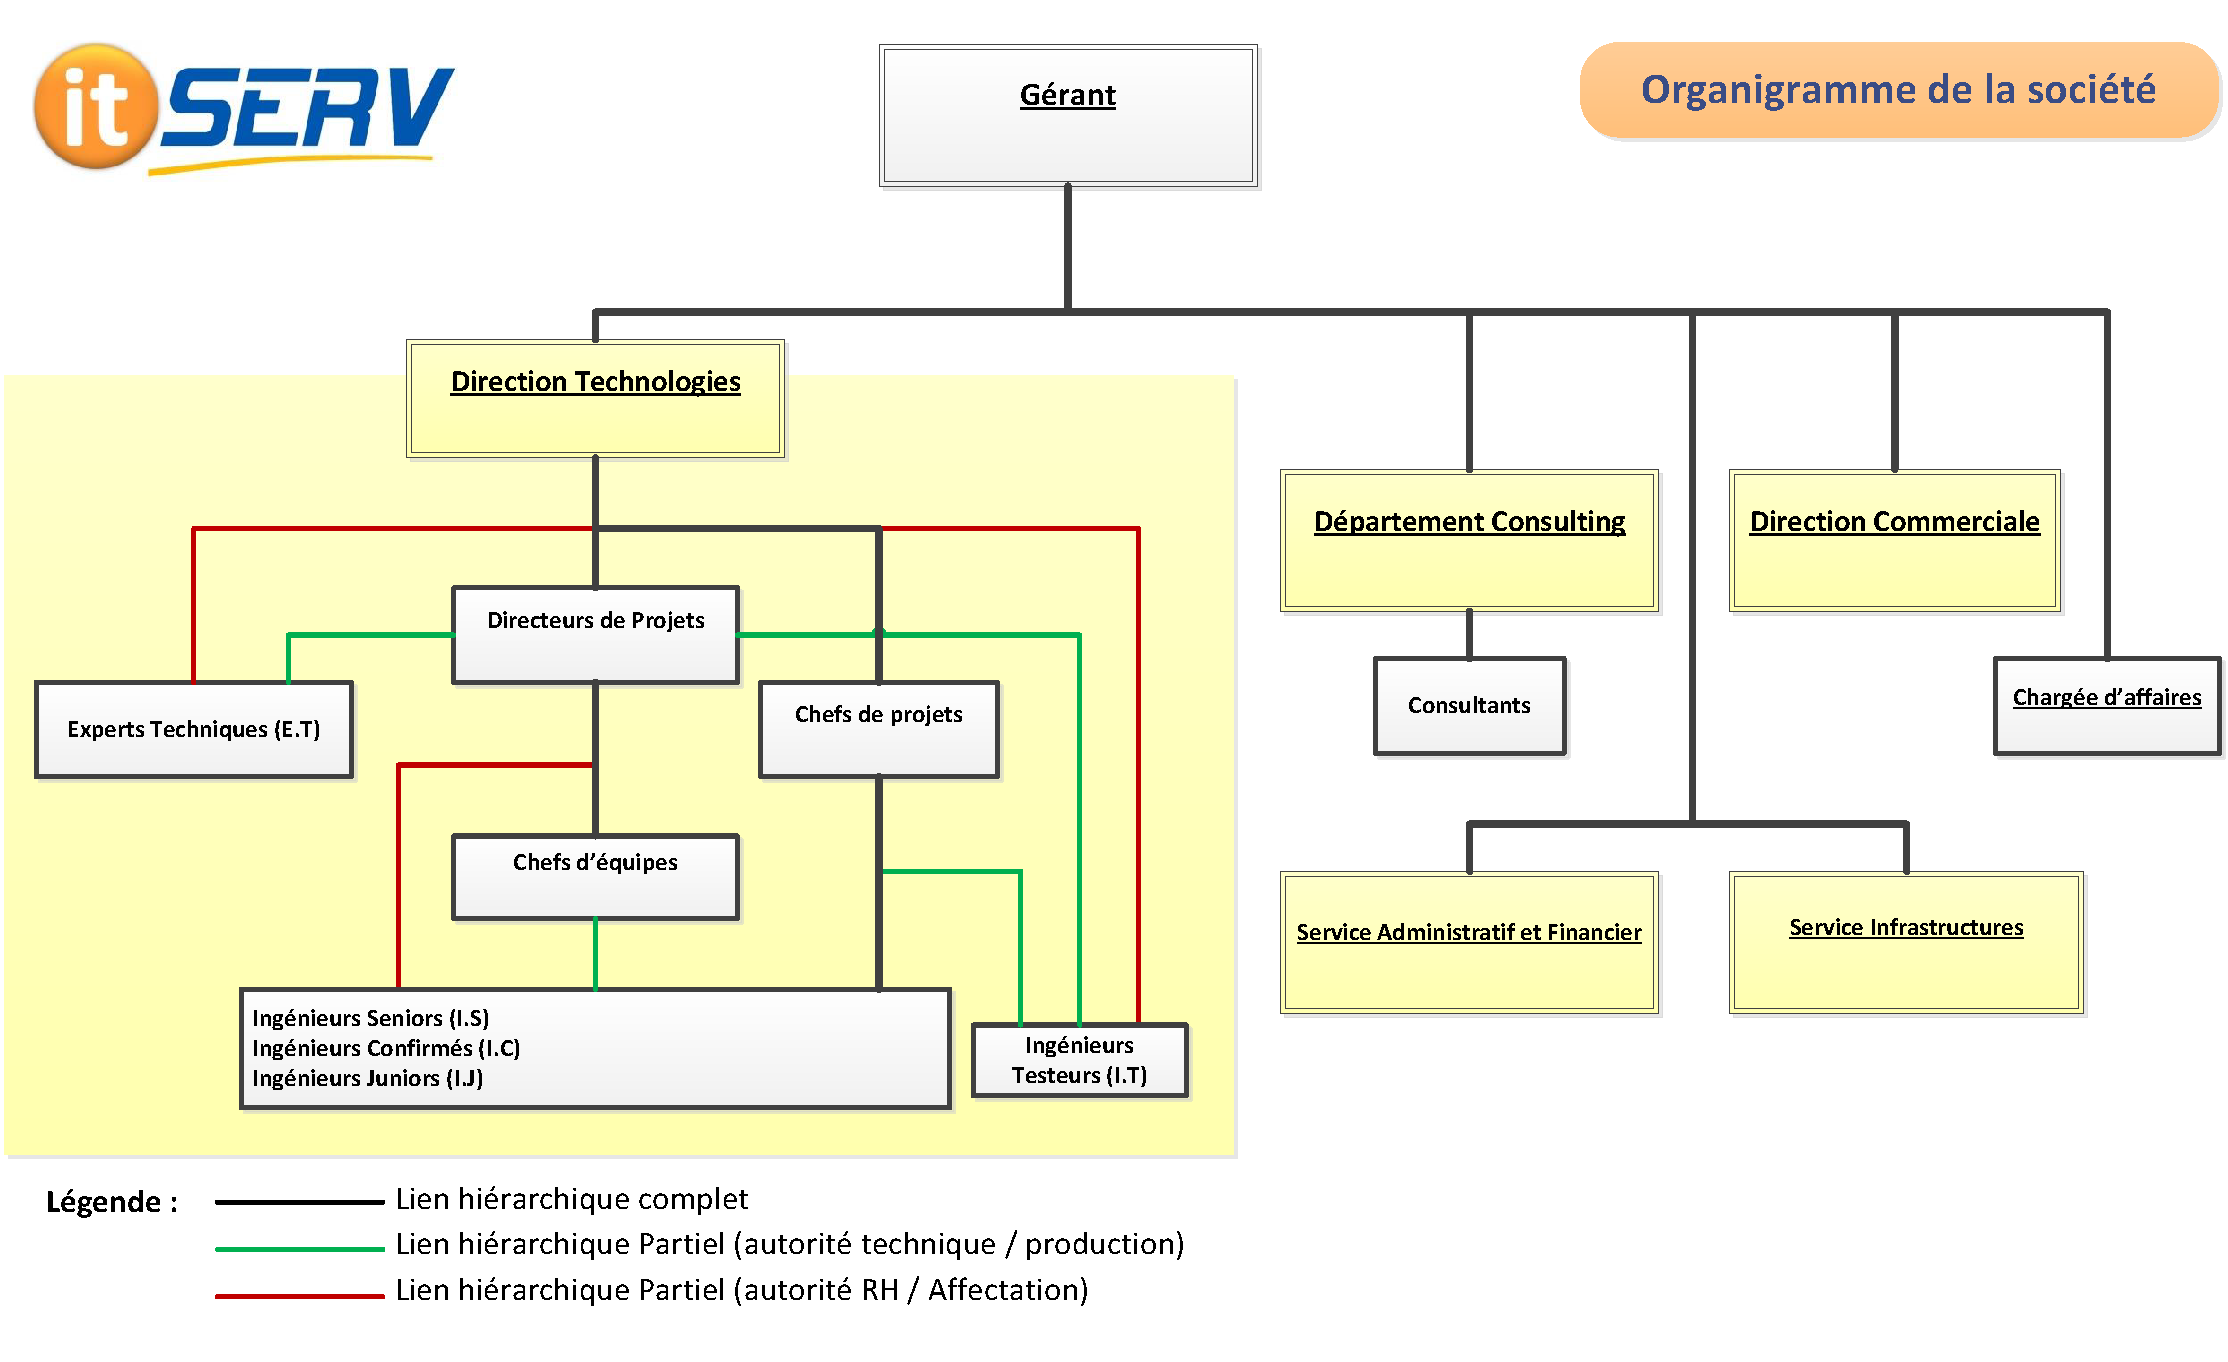
\includegraphics[scale=0.8]{organigramme.png}
\caption{Organigramme de l'entreprise}
\label{organigrammeImg}
\end{figure} 

\subsection{Domaine d'expertise}
Elle est sp�cialis�e dans la d�finition, la conception et l'appropriation des espaces. "UrbaProd" est pr�sente tout  au long du cycle de vie du processus d'optimisation et de conception des lieux afin d'am�liorer la disposition  des collaborateurs :
\begin{itemize}
                                 \item En amont pour le recueil des besoins et le cadrage strat�gique.
                                 \item Puis pour la conception et la r�alisation des plans des espaces.
                                 \item Enfin pour la gestion et le pilotage de mobilit� et l'ing�nierie de transfert.
                               \end{itemize}
Les missions de "UrbaProd" incluent :
\begin{itemize}
  \item Audit et programmation - Concept et charte d'am�nagement - Etudes et space planning.
  \item Prospective - Management de projet - Conduite du changement.
  \item Architecture d'int�rieur - Prescription mobilier - Conduite de travaux.
  \item Pilotage et gestion de la mobilit� - Ing�nierie de transfert.
  \item Solutions num�riques de gestion et visualisation des espaces.
\end{itemize}
"UrbaProd" travaille et accompagne les processus d'am�nagements des grands comptes en France et en Europe, � savoir : EDF, Thales, Cartier, Danone, INPI, l'Or�al, Technicolor, Hachette Livre dont nous retrouvons les logos dans la figure \ref{refenrenceImg}.

\begin{figure}[!ht]
\centering

\includegraphics[scale=0.8]{reference.png}
\caption{R�f�rences de l'entreprise}
\label{refenrenceImg}
\end{figure}

\section{Probl�matique}
Aujourd'hui, nous avons de plus en plus de demandes � traiter, sans avoir un support informatique pour les g�rer. Ce n'est pas tr�s ais� de g�rer l'historique de la client�le d'une entreprise. De plus, lors des diff�rentes int�ractions avec la client�le, et en particulier lors du partage d'informations, l'outils utilis� est le mail. Cependant, cela vire au d�sordre, i.e. messages dissparus, m�thodes de classements qui diff�rent d'un collaborateur � un autre, absence de suivi. Et comme la relation entre collaborateurs est la priorit� strat�gique de la soci�t�, ce point est � travailler d'urgence.

\section{Solutions existantes}
Il existe plusieurs solutions de gestion de relation client sur le march�. En examinant ces applications, nous citons les plus importantes :
\subsection{Version �diteur}
\begin{itemize}

\item[\ding{108}]
\textbf{CRM de Fitnet Manager} : Fitnet Avant-vente est l'outil de gestion commerciale de Fitnet Manager. Les solutions CRM et ERP existent c�tes � c�tes. Activ�es ensemble, elles fonctionnent d'une mani�re enti�rement int�gr�e. Fitnet Manager couvre ainsi l'ensemble du cycle de vie de l'activit� : depuis la prospection jusqu'� la facturation et l'analyse dans les reporting \cite{Fitnet}.

  \item[\ding{108}]
  \textbf{Everwin CXM} : c'est une solution qui vise les cabinets d'architectures, elle couvre plusieurs fonctionnalit�s citant � titre d'exemple :
  \begin{itemize}
    \item
    Base de donn�es de la soci�t� et des contacts avec gestion automatis�e de la t�l�prospection.
    \item
    Gestion des actions commerciales et des campagnes marketing.
    \item
    Agenda partag� et planning g�n�ral des collaborateurs.
  \end{itemize}

\end{itemize}
Cette solution est fond�e sur une technologie Client/Serveur sous windows avec une base de donn�es SQL Server.
il est disponible en mode SaaS ou licence et peut �tre coupl� aux ERP ERPEverwin SX et Everwin GX \cite{Everwin} .   La figure \ref{everwinImg} illustre l'ensemble des fonctionnalit�s couvertes par Everwin CXM.

\begin{figure}[!ht]\centering
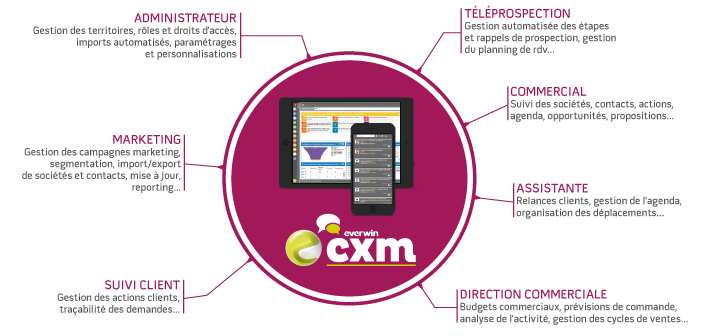
\includegraphics[scale=0.9]{everwinCXM.png}
\caption{Fonctionnalit�s offertes par Everwin CXM \cite{Everwin} }
\label{everwinImg}
\end{figure}

\subsection{Version libre}
 \textbf{Dolibar ERP/CRM} : cette solution g�re les activit�s professionnelles ou associatives de point de vue contact, commandes, stock. Elle g�re aussi la gestion des projets et les avancements de leurs t�ches, et assure m�me la gestion de la ressource humaine.
	Dolibarr est disponible pour toute plate-forme puisqu'elle est d�velopp�e en PHP, MySQL ou encore PostgreSQL .
La figure \ref{dolibarr1Img} illustre l'architecture sur laquelle est bas�e la solution Dolibarr :

\begin{figure}[!ht]\centering
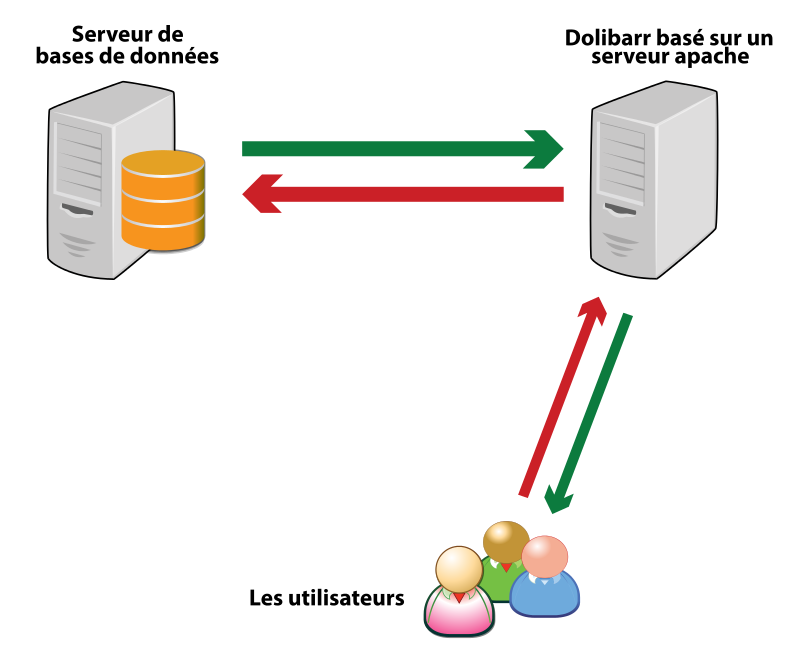
\includegraphics[scale=0.4]{Dolibarr1.png}
\caption{Architecture Dolibarr \cite{Dolibarr} }
\label{dolibarr1Img}
\end{figure}

Pour les non connaisseurs dans le domaine du d�veloppement, il existe un auto-installateur qui se charge d'installer la solution avec tous ses pr�-requis (apache,mysql,php) \cite{Dolibarr}.
La figure \ref{dolibarr2Img} pr�sente l'�cran d'accueil de Dolibarr :

\begin{figure}[!ht]\centering
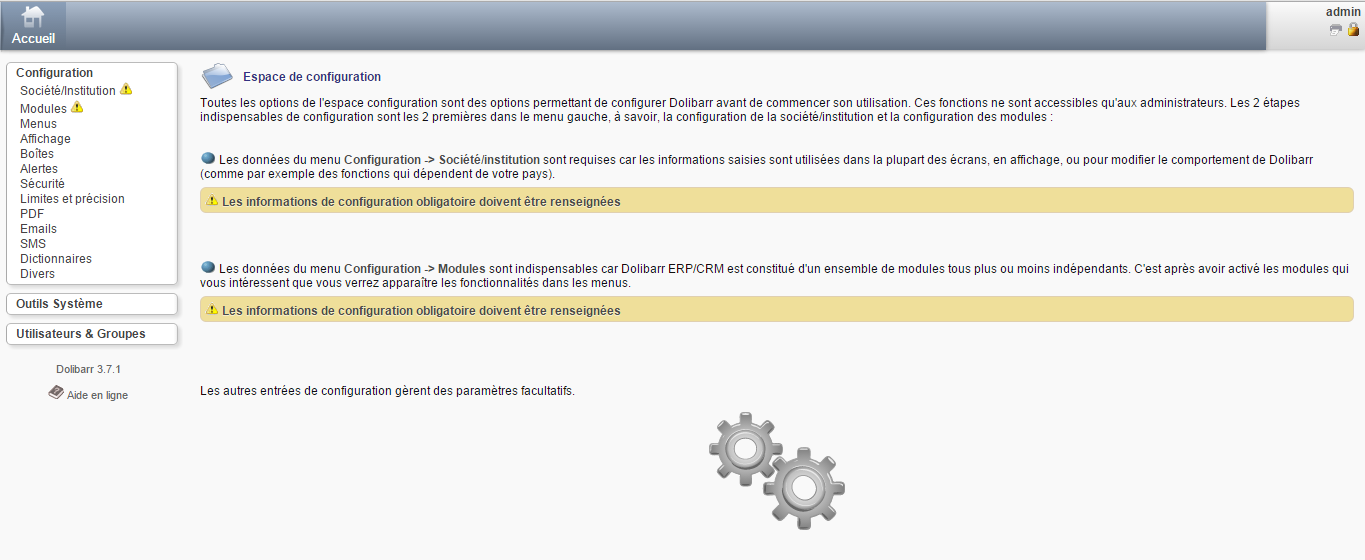
\includegraphics[scale=0.5]{accueil.png}
\caption{Ecran d'accueil de Dolibarr \cite{Dolibarr} }
\label{dolibarr2Img}
\end{figure}

\subsection{Etude comparative}
Le tableau \ref{compSolExt} pr�sente un comparatif entre les solutions existantes pr�sent�es pr�c�demment :

\begin{table}[!ht]\centering
  \centering
  \begin{tabular}{|c|c|c|c|c|c|}
    \hline
    % after \\: \hline or \cline{col1-col2} \cline{col3-col4} ...
    Solution & Payante &  Commentaire & Alertes & Mails & Accueil simple \\
    \hline
    Fitnet & oui  & non & oui & oui & non \\
    \hline
    Everwin CXM & oui  & non & oui & oui & non \\
    \hline
    Dolibarr & non  & non & oui & oui & non \\
    \hline
  \end{tabular}
  \caption{Comparatif entre les solutions existantes}\label{compSolExt}
\end{table}

Les applications �tudi�es, qu'elles soient en versions �diteurs ou m�me gratuites, et malgr� leurs adaptabilit�s et la diversit� de leurs fonctionnalit�s offertes, restent incapable de satisfaire les exigences de la soci�t�. En effet, elles n'int�grent pas un syst�me de commentaire et leur manipulation reste plut�t complexe compar�e � la solution � laquelle nous voulons aboutir.

\section{Objectifs du projet}
Nous voulons offrir un meilleur service dans nos r�ponses aux collaborateurs � l'aide d'un v�ritable outil de gestion des demandes. Aujourd'hui nous visons de :
\begin{itemize}
  \item Faciliter la gestion des demandes.
  \item Rendre l'interaction entre les collaborateurs situ�s en Tunisie et en France plus fluide.
  \item Avoir un syst�me de notification dans l'application, par mail et par sms.
  \item Mesurer leur taux de satisfaction vis-�-vis des r�ponses aux demandes.
  \item Identifier le dysfonctionnement dans notre processus de travail.
  \item Avoir un suivi et une �valuation.
\end{itemize}

\section{Contexte m�thodologique du projet}
La grande �volution dans le domaine du d�veloppement est accompagn�e par une �volution des moyens assurant le bon fonctionnement de ce dernier. D'o� l'apparition des m�thodes agiles permettant d'organiser le cycle de d�veloppement des projets informatiques.

Les m�thodes agiles sont bas�es sur des principes communs d�finis dans l'Agile Manifesto qui est r�dig� par des experts dans ce domaine \cite{AgManifesto}. Ils se reposent essentiellement sur une approche it�rative incr�mentale et adaptative �voluant en parall�le avec les besoins du client, afin de livrer un produit de qualit�.
Il existe plusieurs m�thodes agiles, � savoir, la m�thode  RUP \cite{RUP}, la m�thode XP \cite{XP}, la m�thode SCRUM \cite{SCRUM} et la m�thode RAD \cite{RAD}.

\subsection{Le choix de la M�thode Scrum}
Dans la majorit� des projets, il est difficile d'anticiper les attentes du client. Ceci nous oriente vers une approche it�rative permettant de s'adapter aux exigences du client au fur et � mesure de l'avancement du projet. Pour ce faire, nous avons choisi d'adopter la m�thode Scrum.
Aujourd'hui, Scrum est la m�thode agile la plus utilis�e. Elle permet de produire une solution de la plus haute qualit� dans des bref d�lais.
Cette m�thode est munie des atouts suivants :
\begin{itemize}
  \item Meilleur vue d'ensemble du projet : nous avons une vue globale sur l'avancement du projet par tous les membres des diff�rentes �quipes avec un traitement r�gulier des probl�mes rencontr�s durant chaque phase.
  \item Mise � jour des priorit�s : le client, qui n'est pas n�cessairement un informaticien, n'a pas toujours une vision compl�te sur le produit final. Pour cela, et gr�ce � la composition s�quentielle du contenu des sprints, il b�n�ficie d'une flexibilit� au niveau de la d�finition, de l'�volution des priorit�s et des s�quences d'activit�s.
  \item Qualit� du produit mise en avant : Cette m�thode se repose sur une �valuation r�guli�re du travail, ce qui permet un meilleur traitement des probl�mes (bug), une meilleure productivit� et un produit satisfaisant \cite{AvantageScrum}.
\end{itemize}

\subsection{Les r�les et les notions}
Les r�les dans Scrum :
\begin{itemize}
  \item Le product owner est le responsable du produit. Il est g�n�ralement le client et c'est lui qui exprime les diff�rentes sp�cifications fonctionnelles et leurs priorit�s.
  \item L'�quipe de d�veloppement est responsable de la r�alisation du livrable. Elle est constitu�e par l'entreprise et elle est auto-organis�.
  \item Le scrum master est le premier responsable sur le bon d�roulement des processus de la m�thode scrum.
\end{itemize}

Notion :
\begin{itemize}
  \item Sprint  : une it�ration de travail qui dure entre 15 et 30 jours.
  \item Le product backlog : repr�sente la liste des fonctionnalit�s r�dig�es par le product owner avec tous les correctifs et les am�liorations. Il est donc modifiable tout au long du projet. Le product backlog est pr�sent� sous forme d'items.
  \item Le sprint backlog : est l'ensemble des items planifi�s pour le sprint en cour \cite{SCRUM}.
\end{itemize}


\section*{Conclusion}
Dans ce chapitre, nous avons pr�sent� le cadre g�n�ral du travail, en commen�ant par la pr�sentation de l'entreprise Urbaprod, passant par la probl�matique du projet, ainsi qu'une �tude des solutions existantes sur le march�. Et pour finir, nous avons pr�sent� la m�thode qui va guider notre travail tout au long du projet. Dans le chapitre suivant, nous introduisons les sp�cifications de notre projet.


%==============================================================================
\end{spacing}

%\setcounter{chapter}{1}
\chapter{          ÉTUDE PRÉLIMINAIRE}
\minitoc %insert la minitoc
\graphicspath{{Chapitre2/figures/}}

%\DoPToC

%==============================================================================
\pagestyle{fancy}
\fancyhf{}
\fancyhead[R]{\bfseries\rightmark}
\fancyfoot[R]{\thepage}
\renewcommand{\headrulewidth}{0.5pt}
\renewcommand{\footrulewidth}{0pt}
\renewcommand{\chaptermark}[1]{\markboth{\MakeUppercase{\chaptername~\thechapter. #1 }}{}}
\renewcommand{\sectionmark}[1]{\markright{\thechapter.\thesection~ #1}}

\begin{spacing}{1.5}

%==============================================================================
\section*{Introduction}
Après avoir présenté le cadre général de notre projet, nous entamons par le biais de ce chapitre une étude théorique, préface à sa réalisation. Nous commençerons par présenter les notions de base associées à la partie métier du projet. Nous enchaînerons avec l'étude de l'existant, qui sera l'opportunité de présenter plus en détail la problématique rencontrée en interne par l'entreprise. Enfin, une vue d'ensemble des solutions similaires présentes sur le marché permettra de se faire une idée globale sur les fonctionnalités à attendre du produit.\\
Cette étude, partie intégrale de l'élaboration de la vision initiale du produit, s'inscrit dans la phase d'inception de la méthodologie de travail adoptée.


%==============================================================================
\section{La Gestion de Projet}
Les entreprises se confrontent à de nombreux challenges au cours de leur évolution (adaptation à des contraintes externes, lancement de nouveaux services ou produits, intégration de nouveaux outils, mises à jour des processus, ...). Chaque défi est relevé sous forme de projet. Un projet est défini sous forme d'une suite d'actions délimitée dans le temps, en vue de produire un résultat spécifique, un produit, un service ou une nouvelle organisation.\\
La gestion de projet a pour vocation de relever ces défis en mettant en place une organisation et une planification de l’ensemble des activités visant à assurer l’atteinte des objectifs du projet (qualité, coûts, délais, ...), à effectuer leur suivi, anticiper les risques et les changements à mettre en œuvre  ainsi qu'à gérer la communication et la prise de décision.\\
\\
On peut regrouper les activités de gestion de projet en deux phases :
\begin{itemize}
%    \item \textbf{} :
    \item La phase d'organisation
    \item La phase de pilotage
\end{itemize}
\\
Ces activités sont précédées par une phase de collecte d'informations et d'étude de faisabilité. Cette phase d'avant projet permet de valider le projet et de décider des ressources à mobiliser pour sa mise en œuvre.
% REF: http://ressources.aunege.fr/nuxeo/site/esupversions/6b35be1e-5317-4cd6-8db2-05485615219d
% REF: http://www.gestiondeprojet.net
%-----------------------------------------------------------------------------------
\subsection{Phase d'organisation}
La phase d'organisation comprend le développement des concepts définis dans la phase d'avant projet et la définition du référentiel du projet, en fournissant suffisamment de détails pour pouvoir entamer la phase de réalisation. Les principaux éléments du référentiel d'un projet incluent :
\begin{itemize}
%    \item \textbf{} :
    \item \textbf{La charte du projet} : Elle est rédigée par le chef de projet dès son lancement. Elle est destinée à toutes les personnes appelées à travailler sur le projet, ainsi qu'aux tiers concernés (la hiérarchie, les chefs de service, ...). C'est un document de référence à usage strictement interne dont le but est de fournir les informations de base du projet : son objet, ses parties prenantes, ses enjeux, ses contraintes, etc.
    \item \textbf{La structuration du projet} : La structure de découpage du projet organise et définit la totalité du contenu d'un projet. La structuration du projet dépend de nombreux paramètres (la complexité, la structure de l'organisation, le type de gestion, ...) et a pour objectif de découper le projet en plus petits éléments, plus faciles à gérer, afin de pouvoir définir des coûts et des durées pour chaque élément, ainsi que des résultats tangibles et mesurables.
    \item \textbf{Le planning de référence} : La planification d'un projet est l’activité qui consiste à déterminer et à ordonnancer les tâches du projet, à estimer leurs charges et à déterminer les profils nécessaires à leur réalisation. Le planning résultant inclut la liste des tâches et leurs antériorités, la définition des lots de travaux ainsi que les ressources associées.
    \item \textbf{Le plan de communication} : C'est un document qui présente les méthodes et les modalités adoptées pour collecter, conserver et diffuser l'information, les destinataires de chaque type d'information (rapport, document technique, ...), ainsi que les responsabilités associées.
    \item \textbf{Le budget de référence} : Résultat de l'analyse des coûts rattachés au projet, il est établi à partir de la liste des activités, des ressources associées et du planning de référence.
    \item \textbf{L'analyse des risques} : Elle comporte un recensement des aléas majeurs associés au projet ainsi que les plans d'action et les mesures préventives à mettre en place.
\end{itemize}

%-----------------------------------------------------------------------------------
\subsection{Phase de pilotage}
Une fois budgétisé, organisé et planifié, le projet démarre. Le pilotage du projet permet de comparer le réalisé avec le prévisionnel, et de réviser éventuellement les plannings et les charges. Le chef de projet et son équipe s'efforcent de respecter le référentiel de gestion du projet, tout en mesurant les écarts constatés. Cela inclut la maîtrise des aspects suivants :
\begin{itemize}
%    \item \textbf{}} :
    \item \textbf{Les délais} : Le chef de projet recueille l'information sur l'avancement réel du projet à partir de l'avancement de chaque tâche, et identifie les retards actuels et potentiels. Dès lors, des actions correctives peuvent être mises en place afin de corriger les écarts (modification du planning, réallocation de ressources, ...).
    \item \textbf{Les coûts} : Une évaluation de la consommation budget est fréquemment entreprise, suivie d'une réestimation du budget qui reste à consommer. Le coût total prévu comparé au budget de référence permet d'analyser et d'anticiper des écarts ainsi que d'identifier les causes de dépassement.
    \item \textbf{Les modifications} : Elles sont le résultat d'événements extérieurs (changement de réglementation, changement demandé par le client, erreurs ou oublis dans la définition initiale, ...). Les demandes de changements peuvent apparaître sous plusieurs formes et conduire à un élargissement ou à une limitation du contenu et doivent être traitées grâce un ensemble de procédures formelles.
    \item \textbf{Les risques} : La maîtrise des risques permet d'identifier, de quantifier, de réduire ainsi que de suivre les risques encourus tout au long de la vie du projet.
\end{itemize}
Le chef de projet se focalise essentiellement sur la maîtrise des coûts et des délais.\\

L'usage d’indicateurs de pilotage est crucial pour le pilotage efficace d'un projet. Ces outils d'assistance à la décision permettent de mesurer de manière pratique une situation ou un risque, d'alerter ou au contraire de signifier l'avancement correct d'un projet.


%==============================================================================
\section{Étude de l'existant}
L'étude de l'existant permet d'identifier les points forts ainsi que les points faibles de la solution existante. Cette étude permettra de bien cibler les besoins de l'entreprise, en vue d'en tenir compte lors de la conception et du développement de la solution.
%-----------------------------------------------------------------------------------
\subsection{Description de l'existant}
La solution de gestion de projet actuelle se base sur l'utilisation du logiciel Excel pour générer des documents associés aux différentes activités d'un projet. En effet, le chef de projet répertorie chaque catégorie d'artéfact associée à la gestion d'un projet sous forme de tableur Excel. Il procède ainsi à l'ajout et l'édition d'entrées pour chaque catégorie d'artéfact et y indique l'ensemble des informations requises. Cette procédure est facilitée par la duplication de fiches Excel de base, vierges, préparées à l'avance pour chaque catégorie. Ainsi, pour chaque catégorie d'artéfact, l'ensemble des entêtes et des valeurs prédéfinies pour chaque champs y est déja déclaré. La table d'entrées d'une fiche est souvent accompagnée d'un ensemble d'indicateurs, statiques et dynamiques, pertinents à la catégorie en question. Des exemples de ces fiches sont exposés aux figures \ref{fig:risqueFiche} et \ref{fig:actionFiche}, traitant respectivement des artéfacts actions et risques pour un projet.

\begin{figure}[H]
\centering
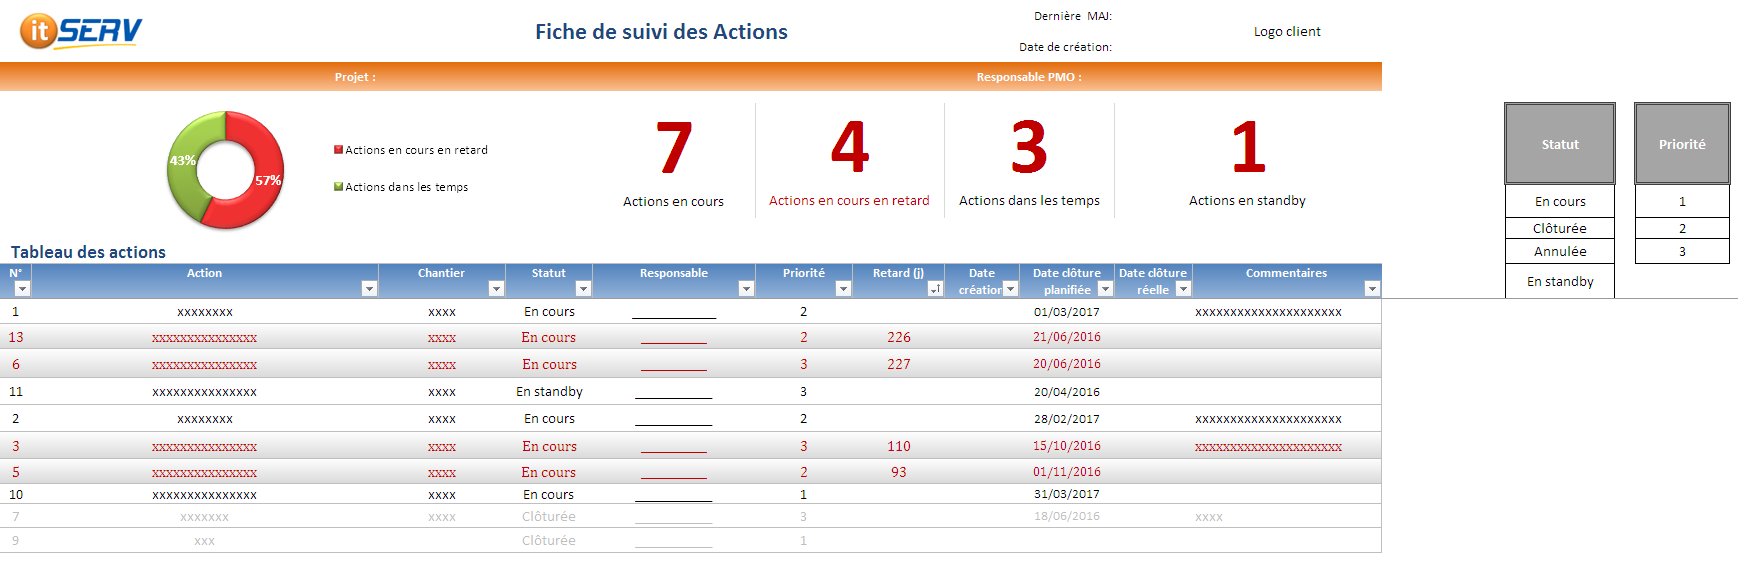
\includegraphics[width=\linewidth]{ficheActions.png}
\caption{Exemple d'une fiche de suivi des actions}
\label{fig:actionFiche}
\end{figure}

\begin{figure}[H]
\centering
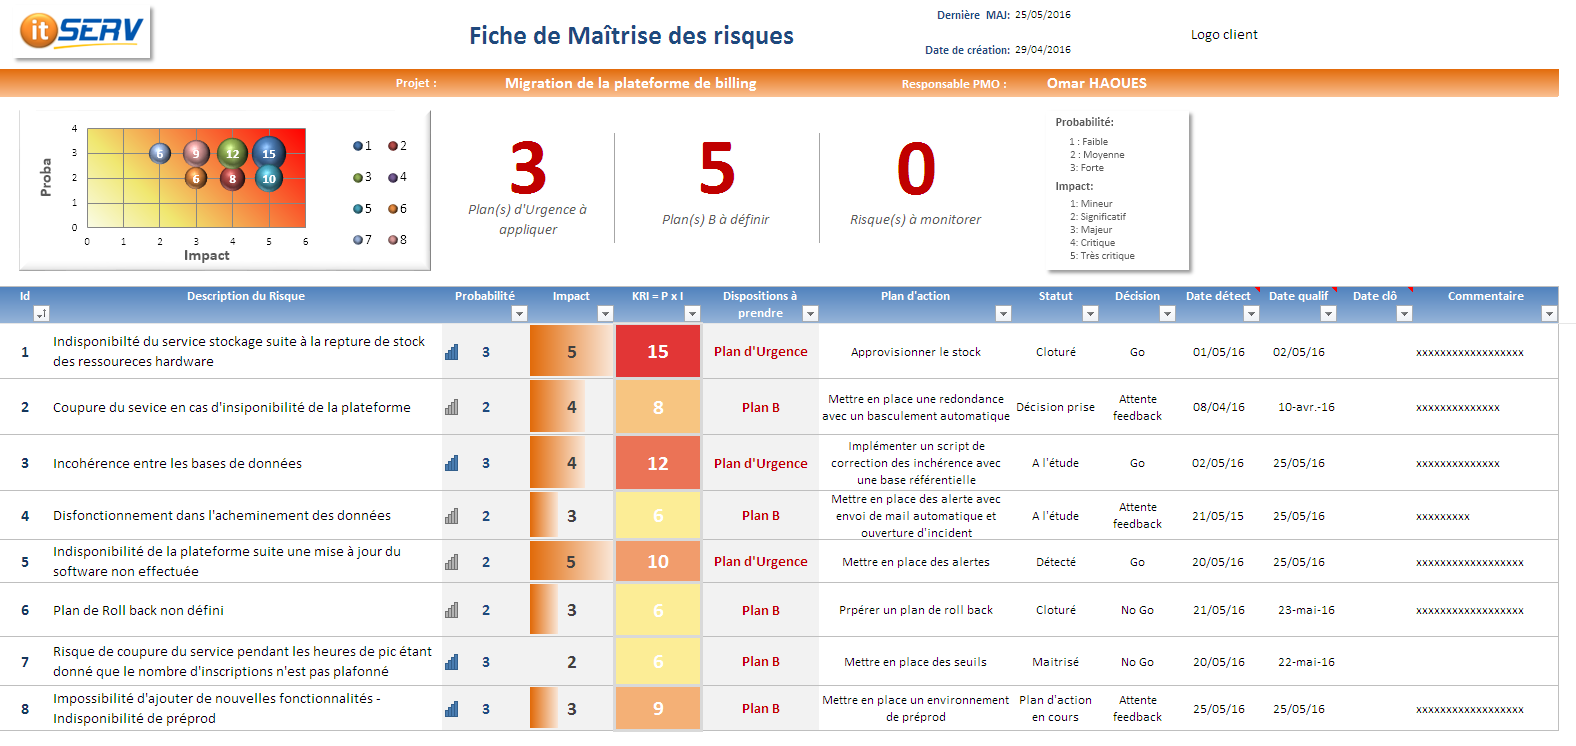
\includegraphics[width=\linewidth]{ficheRisques.png}
\caption{Exemple d'une fiche de maîtrise des risques}
\label{fig:risqueFiche}
\end{figure}
\

Le chef de projet est régulièrement chargé de diffuser les mises à jour relatives à un projet, périodiquement ou à la demande, au travers de l'envoi de messages électroniques directement aux parties concernées.\\

Cette méthode de travail possède certains atouts, mais dissimule dans l'ensemble plusieurs inconvenances qui nuisent à son niveau d'efficacité et à la performance de la gestion de projets par l'entreprise. Ces points sont exposés dans la section suivante.

%-----------------------------------------------------------------------------------
\subsection{Critique de l'existant}
La présentation de la méthode de gestion actuelle nous permet de déceler des limitations importantes, inhérentes à la démarche générale.\\
\\
Reconnaissons tout d'abord les mérites non négilgeables de celle-ci, à savoir :
\begin{itemize}
    \item Disponibilité de fiches de base, contraignant les champs à choix restraints aux options prédéfinies et assistant à leur remplissage
    \item Présence de champs autocalculés ainsi que de supports visuels utiles pour la compréhension de certains champs, dont la signification peut s'avérer obscure
    \item Génération automatique d'indicateurs riches (statistiques numériques, graphiques en camembert, ...)
\end{itemize}
\

Outre ces quelques bénéfices, cette méthode de gestion présente les nombreuses limitations suivantes :
\begin{itemize}
    \item \textbf{Perte en productivité} : induite d'un déficit d'automatisation de la démarche de gestion des fichiers
    \item \textbf{Fragmentation des données} : les données relatives à chaque projet sont réparties, sous forme d'une multitude de documents, souvent désorganisés
    \item \textbf{Journalisation non fiable des mises à jour} : la journalisation des mises à jours relève entièrement de l'organisation choisie par le chef de projet, et requiert un effort manuel, exclusivement dédié à la tâche
    \item \textbf{Traçabilité impossible} : l'origine des modifications des fichiers n'est pas connue
    \item \textbf{Stockage inneficace} : problème de centralisation pour l'ensemble des données des projets menés par l'entreprise, redondance de données, oraganisation manuelle, etc
    \item \textbf{Sécurité non garantie} : la sécurisation des données (documents) est entièrement à la charge des parties prenantes y ayant accès
    \item \textbf{Condifentailité difficile à assurer} : elle implique en pratique l'édition soigneuse, au cas par cas, des fichiers partagés
    \item \textbf{Synthèse des données impossible} : impossible de se reposer fiablement sur les données des fichiers pour les besoins d'aide à la décision de l'entreprise (à cause des points susmentionnés)
    \item \textbf{Collaboration fastidieuse} : contribution d'intervenants non gérée par la solution actuelle. Le chef de projet transforme individuellement tous les flux d'information en données, avant de les indiquer dans le fichier approprié
\end{itemize}
\

Toutes les limitaions susmentionnées imposent pour l'entreprise une révolution dans sa méthode actuelle de gestion de projets. Dans le cadre de notre projet de fin d'études, la solution à concevoir aspire ainsi à combiner les points forts de la démarche existante tout en apportant une solution efficace à ses problèmes inhérents.


%==============================================================================
\section{Étude des solutions existantes sur le marché}
Le problème de gestion de projet est aussi vieux que le concept de projet lui-même. En conséquence, un nombre important de solutions logicielles d'aide à la gestion de projet est disponible aujourd'hui sur le marché. Dans le but de produire une solution de qualité, une étude de l'existant s'impose afin de prendre en considération les points forts et les points faibles des solutions existantes. Celle-ci servira surtout à nous guider dans l'élaboration de la vision de notre produit.

%-----------------------------------------------------------------------------------
\subsection{Présentation des solutions existantes}
Les solutions présentes sur le marché se distinguent les unes des autres essentiellement par le niveau de fonctionnalités offert et le domaine d'application cible. En effet, des solutions populaires, telle que JIRA \ref{JIRA}, se limitent à un domaine très particulier, en l'occurence la gestion de projets agiles pour cette dernière. Les solutions étudiées aspirent à être le plus générique possible, capable d'être employées dans n'importe quel contexte de projet. L'échantillon exposé ci-dessous vise à présenter une vue d'ensemble des caractéristiques communes et distinctives des solutions les plus populaires sur le marché qui partagent cette vision.

\subsubsection*{MS Projects} %-------------------------------------------------------------------------
Microsoft Projects a su s'imposer pendant longtemps en tant que solution de facto pour les besoins de gestion de projet en entreprise. Faisant partie de la suite logicille de l'éditeur, MS Projects ne fait pas exception et s'intègre pleinement à sa plateforme collaborative \ref{Office 365}, ce qui représente un réel bénéfice pour les clients ayant déja opté pour l'intégration de leurs données sur cette dernière. Le logiciel continue d'introduire un nombre de fonctionnalités avancées avec ses mises à jour. Ceci le rend particulièrement adapté aux besoins poussés de gestion de projet. Les utilisateurs expérimentés y trouvent leur compte, cependant la courbe d'apprentisage est souvent pénible pour les novices et s'avère être trop complexe pour les usages se limitant en besoin à un nombre restreint de ses fonctionnalités.

\subsubsection*{ProjectManager.com} %------------------------------------------------------------------
ProjectManager.com couvre très bien les fonctionnalités de base de gestion de projet et, parmi toutes les solutions étudiées, s'apparente le plus à la vision initiale élaborée. Cette solution, disponible sous une offre SaaS \ref{SaaS}, s'adapte parfaitement aux besoins des petites et moyennes entreprises, qui retrouvent une simplicité d'usage associée à une couverture plus que décente des piliers de la gesion professionnelle de projet.

\subsubsection*{Zoho Projects} %-----------------------------------------------------------------------
Zoho propose une suite logicielle qui répond aux besoins des particuilers et des entreprises. Dans cette optique, sa solution de gestion de projet s'intègre parfaitement avec certains de ses autres produits, afin d'étendre ses fonctionnalités. La solution se veut simple, mais complète, en offrant un éventail éttoffé de fonctionnalités pour la gestion des divers facettes d'un projet. Elle se caractérise par une attention particuière apportée à l'ergonomie et au confort général d'utilisation.

\subsubsection*{EasyProject (EasyRedmine)} %-----------------------------------------------------------------------------
Redmine est la solution open source gratuite la plus complète disponible sur le marché. Cependant, son manque d'intuitivité et le faible niveau d'ergonomie offert, associés à son interface datée, nuisent à son potentiel et en font une solution peu courante d'usage dans la pratique. C'est tout d'abord dans le but d'accroître son utilisabilité, tout en prenant avantage de la base de fonctionnalités existante, que la solution EasyProject offre une version commerciale, basée sur cette solution. Depuis, l'application s'est vu évoluer vers l'une des solutions les plus abouties du marché, visant à s'aligner avec les standards de gestion de projets IPMA et PMI.

\subsubsection*{Clarizen} %-----------------------------------------------------------------------------
Due à l'amélioration continue de son produit et à la complétude de sa vision, l'entreprise Clarizen a vu son produit se hisser à la position de Leader dans dans les classements Gartner et Forrester de 2016 \ref{clarizen.com}, dans la catégorie des solutions SaaS de gestion de projets. De ce fait, ce produit a sans nul doute sa place dans notre étude et impose un bilan des traits caractéristiques qui lui valent son succès.
\\

Dans le but de présenter un échantillon pertinent, d'autres solutions ont été omises, notamment pour des raisons de redondance ou de pauvreté en termes de fonctionnalités. Nous poursuivons avec la mise en relief des points communs et distinctifs de chacune dans la partie qui suit.

%-----------------------------------------------------------------------------------
\subsection{Synthèse des solutions existantes}

Le tableau \ref{tab:} présente une comparaison haut niveau des solutions étudiées. On y observe que les solutions retenues partagent un tronc commun de fonctionnalités destiné à la gestion des aspects primordiaux d'un projet. Elles se différencient néanmoins sur d'autres points, tel que la nature de l'offre et le support de l'accès mobile.

\begin{table}[h]
\centering
\caption{Comparatif des solutions de gestion de projet présentées}
\label{comparatifSolutionsEtudiees}
\begin{tabularx}{1\textwidth}{|p{4cm}|1|1|1|1|1|}
\hline
        \textbf{Spécificités} & \textbf{MS Proj.} & \textbf{P.M .com} & \textbf{Zoho Proj.}&  \textbf{EasyProject} & \textbf{Clarizen}\\
\hline
        \textbf{Nature d'offre} & Bureau & SaaS & SaaS & SaaS \& Local & SaaS\\
\hline
		\textbf{Planification} & \cmark & \cmark & \cmark & \cmark & \cmark\\
\hline
		\textbf{Gestion Budget} & \cmark & \cmark & \cmark & \cmark & \cmark\\
\hline
		\textbf{Structuration} & \cmark & \cmark & \cmark & \cmark & \cmark\\
\hline
		\textbf{Gestion Ressources} & \cmark & \cmark & \cmark & \cmark & \cmark\\
\hline
		\textbf{Gestion Problèmes} & \cmark & \cmark & \cmark & \cmark & \cmark\\
\hline
        \textbf{Gestion} & \multirow{2}{*}{\xmark} & \multirow{2}{*}{\cmark} & \multirow{2}{*}{\cmark} & \multirow{2}{*}{\cmark} & \multirow{2}{*}{\cmark}\\
        \textbf{Modifications} &  &  &  &  & \\
\hline
		\textbf{Reporting} & \cmark & \cmark & \cmark & \cmark & \cmark\\
\hline
		\textbf{GED} & \cmark & \cmark & \cmark & \cmark & \cmark\\
\hline
		\textbf{Pilotage Risques} & \cmark & \cmark & \cmark & \cmark & \cmark\\
\hline
		\textbf{Support Mobile} & \xmark & Web & App & App & App\\
\hline
		\textbf{Collaboration} & \xmark & \cmark & \cmark & \cmark & \cmark\\
\hline
		\textbf{Open Source} & \xmark & \xmark & \xmark & \cmark & \xmark\\
\hline
\end{tabularx}
\end{table}
\

Vu son expertise en développement d'applications, IT SERV a choisi de démarrer le développement de sa propre solution d'aide à la gestion de projet. Dans le cadre de notre projet de fin d'études, nous visons à concevoir une solution s'inspirant d'une sélection des traits jugés primordiaux des solutions étudiées. Ceux-ci seront établis dans le chapitre \ref{chap: spécs}.

%==============================================================================
\section*{Conclusion}
Afin de mieux cerner la problématique et de proposer une solution de qualité, tenant compte des spécificités de notre projet, nous avons établi l'état des lieux de l'existant, que ce soient les méthodes de gestion courantes de l'entreprise, ou les solutions similaires disponibles sur le marché.\\
Avec ces informations en main, le chapitre suivant nous permettra de dégager précisément les exigences de notre produit.


%==============================================================================
\end{spacing}



\backmatter
\pagestyle{fancy}
\fancyhf{}
\renewcommand{\chaptermark}[1]{\markboth{Conclusion G�n�rale et Perspectives}{}}
\fancyhead[R]{Conclusion G�n�rale et Perspectives}
\fancyfoot[R]{\thepage}
\renewcommand{\headrulewidth}{0.5pt}
\renewcommand{\footrulewidth}{0pt}
%\chapter{Conclusion G�n�rale et Perspectives}
%==============================================================================
\pagestyle{fancy}
\fancyhf{}
\fancyhead[R]{\bfseries\rightmark}
\fancyfoot[R]{\thepage}
\renewcommand{\headrulewidth}{0.5pt}
\renewcommand{\footrulewidth}{0pt}
\renewcommand{\chaptermark}[1]{\markboth{\MakeUppercase{\chaptername~\thechapter. #1 }}{}}
\renewcommand{\sectionmark}[1]{\markright{\thechapter.\thesection~ #1}}

\begin{spacing}{1.5}
%==============================================================================

Dans une entreprise, la gestion des commandes re�ues est une �tape primordiale dans le processus, de conception et/ou de production. C'est l'�tape au cours de laquelle l'�coute du client est importante afin de bien comprendre ses besoins et de tenir compte de ses envies. Gr�ce � l'informatique, nous avons  pu r�pondre � cette probl�matique en utilisant le Customer Relationship Manager (CRM) qui est d�fini comme �tant l'ensemble des outils et techniques permettant de traiter et d'analyser toutes les informations relatives aux clients dans le but de les fid�liser en leur offrant les meilleurs services

Mais, comme toute solution, le CRM souffre d'un ensemble d'inconv�nients. Parmi eux, surgit le probl�me de la facilit� d'utilisation surtout pour les non-connaisseurs, comme les architectes. Nous avons donc pens� � une adaptation du concept du CRM aux besoins d'un architecte qui est une personne peu connaisseuse en informatique.
Dans ce cadre, nous avons effectu� ce stage de fin d'�tude dans la soci�t� � UrbaProd �. Nous �tions charg� de concevoir une plateforme de CRM qui permet, � la fois, de g�rer les demandes des clients en un laps de temps raisonnable, et de sauvegarder l'historique des diff�rentes demandes pass�es par le client. Notre plate-forme devra en plus �tre facile � utiliser par tous les utilisateurs, que ce soient des clients ou des architectes.
Afin d'atteindre ces objectifs, nous avons utilis� le "Framework" Symfony2. Il assure une grande performance et une facilit� d'extensibilit�, nous avons exploit� les composantes qu'il offre comme la gestion de s�curit� pour l'authentification et les droits d'acc�s.
A la fin de ce travail, nous avons r�pondu aux besoins de la soci�t� � travers l'ensemble des fonctionnalit�s fournies par notre solution, � savoir, le module de gestion des demandes, le module de notification et le module de gestion des clients.
Mais cela n'emp�che que nous avons connu quelques difficult�s pendant la p�riode de la collecte des besoins et des difficult�s pendant la p�riode de l'impl�mentation de la solution puisque l'entreprise ne comprend pas dans son effectif des sp�cialistes dans ce domaine.
L'utilisation de Symfony2 facilitera ensuite l'int�gration des am�liorations envisag�s par la soci�t� comme la notification par sms afin de garantir la visibilit� de l'information par tous les collaborateurs. M�me si nous avons utilis� des interfaces responsives, nous avons propos� d'impl�menter une application mobile qui sera plus ad�quate pour les smartphones.

%==============================================================================
\end{spacing} 


%\bibliographystyle{apalike-fr}
\bibliographystyle{Biblio/unsrt_modif}
%\singlespacing
\renewcommand{\bibname}{Bibliographie}

\bibliography{Biblio/aesm_edspia}

\onehalfspacing

\appendix
%\setcounter{figure}{0}
\setcounter{table}{0}
\setcounter{footnote}{0}
\setcounter{equation}{0}
\pagestyle{fancy}
\fancyhf{}
\renewcommand{\chaptermark}[1]{\markboth{\MakeUppercase{#1 }}{}}
\renewcommand{\sectionmark}[1]{\markright{\thesection~ #1}}
\fancyhead[RO]{\bfseries\rightmark}
\fancyhead[LE]{\bfseries\leftmark}
\fancyfoot[RO]{\thepage}
\fancyfoot[LE]{\thepage}
\renewcommand{\headrulewidth}{0.5pt}
\renewcommand{\footrulewidth}{0pt}

\makeatletter
\renewcommand\thefigure{A.\arabic{figure}}
\renewcommand\thetable{A.\arabic{table}}
\makeatother

\chapter{Annexe : Remarques Diverses - BIDON}
\graphicspath{{Annexe1/figures/}}
%==========================================================================

%    Annexe

%===========================================================================

\begin{figure}[!ht]
\centering

\includegraphics[scale=1]{ingenieur.jpg}
\caption{Demande sous sa forme originale}
\label{demOrgForm}
\end{figure} 


\end{document} 